\documentclass[a4paper]{article}

\usepackage{fullpage} % Package to use full page
%\usepackage{parskip} % Package to tweak paragraph skipping
%\usepackage{tikz} % Package for drawing
\usepackage{graphicx}
\usepackage{amsmath}
\usepackage{hyperref}%}[hidelinks]{hyperref}
\hypersetup{linkcolor=blue}
\usepackage{floatrow} %Put caption next to figure
\usepackage{float} %Put caption next to figure
%\usepackage{multicol}
%\setlength{\columnsep}{1cm}


\title{
\vspace{-3ex}Informe Hipparcos\\
\vspace{1ex}
\large An\'{a}lisis de las estrellas localizadas a una distancia menor de 10 parsecs}

\author{Ignacio Hern\'{a}ndez-Ros Bellosillo}
\date{\vspace{-1ex}}

\setlength{\parindent}{12pt}
\begin{document}

\maketitle

\section{Resultados Obtenidos. Comentarios generales}

	\hspace*{12pt}En el siguiente trabajo se analizar\'{a}n las propiedades b\'{a}sicas de las estrellas que se encuentran a una discancia menor de 10 pc de nosotros. Para ello se han discriminado de la base de datos obtenidos por el satélite Hipparcos las estrellas cuyo paralaje es mayor de 0.1 segundos de arco. Los resultados obtenidos de los datos son los que siguen:

	\subsection{Distribuci\'{o}n de luminosidad}
	
		\hspace*{12pt}Los resultados obtenidos para la luminosidad de cada estrella en la vecindad solar son los que siguen:

	\begin{figure}[!htbp]
		\centering
		\title{\textbf{Histograma de luminosidades}}
		\begin{center}
			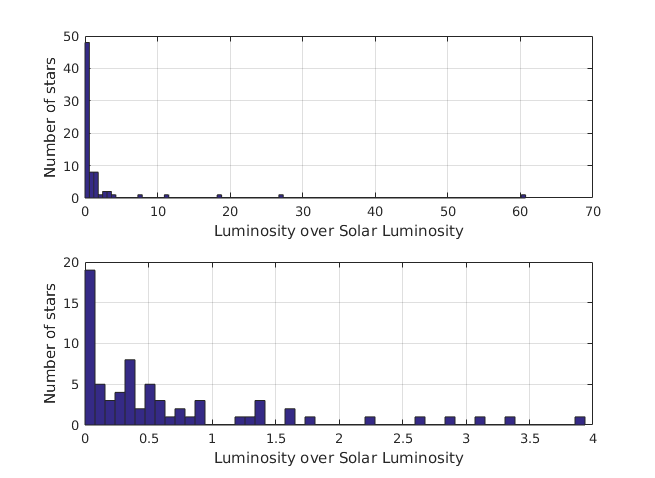
\includegraphics[width=15cm]{Figures/Lhist.png}
		\end{center}
		\caption{\footnotesize{
		Distribuci\'{o}n obtenida para la muestra. En la \textit{Figura 1.1} (Arriba) se muestra el n\'{u}mero de estrellas con una determinada luminosidad comparada con la luminosidad del Sol. En la \textit{Figura 1.2} (Abajo) se ha representado el mismo gr\'{a}fico para el subconjunto muestral mayoritario, el cual se distribuye alrededor de la luminosidad del sol.}}
		\label{Lhist}
	\end{figure}

	Como se puede observar en la Figura \ref{Lhist}, la gran mayor\'{i}a de las estrellas en la vecindad solar emiten con una luminosidad menor a la del Sol. En concreto, m\'{a}s del 50\% de las estrellas presentan una luminosidad menor que la mitad de la luminosidad solar. M\'{a}s adelante, en la Figura \ref{HRdiag}, se explica c\'{o}mo esto est\'{a} relacionado la selecci\'{o}n de estrellas restingida en los tipos espectrales A, F, G y K y el tiempo de vida media caracter\'{i}stico de cada tipo espectral.

	\subsection{Diagrama HR}

		\hspace*{12pt}Los resultados obtenidos para el diagrama HR en la vecindad solar es el que sigue:
	
	\begin{figure}[!htbp]
		\centering
		\title{\textbf{HR Diagram\vspace{2ex}}}
		\begin{center}
			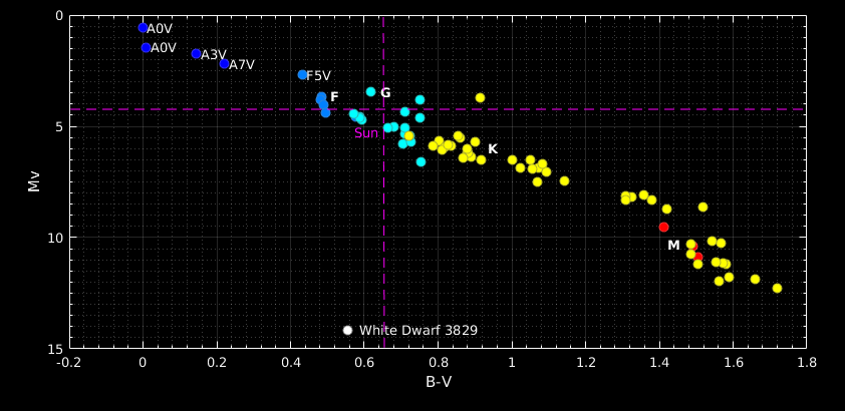
\includegraphics[width=15cm]{Figures/HRdiagram2.png}
		\end{center}
		\caption{\footnotesize{En el siguiente diagrama se han representado ambas cantidades en "magnitudes". Se ha diferenciado el tipo espectral de cada estrella mediante el color del punto que la representa y se ha marcado como referencia la posici\'{o}n del Sol en el diagrama.}}
		\label{HRdiag}
		\end{figure}
		
	Para hacer un an\'{a}lisis de los resultados obtenidos conviene fijarse en los cuadrantes delimitados por las l\'{i}neas solares (Sun en la Figura \ref{HRdiag}). Lo primero que destaca en esta separaci\'{o}n es la diferencia que hay en el n\'{u}mero de estrellas en los cuadrantes superior izquierdo e inferior derecho. Esto puede explicarse facilmente si se tiene en cuenta la vida media asociada a las estrellas de tipo A y F frente a la vida media de las estrellas de tipo K. En general, las estrellas de tipo A y F tienen una vida media mucho menor que las de tipo K, lo que explica c\'{o}mo una distribuci\'{o}n que podemos postular aleatoria de estrellas inicial acaba por consistir en un gran n\'{u}mero de estrellas K y un menor n\'{u}mero del resto seg\'{u}n las de tipo A y F van consumiendose.
	\\ \hspace*{12pt}  Por otro lado, el Sol es una estrellade tipo G, como podemos ver en el diagrama. Esto explica la distribuci\'{o}n de luminosidades obtenida en la Figura \ref{Lhist} donde la gran mayor\'{i}a de estrellas se situaban en una luminosidad menor a la del Sol, lo que equivale a estar en los cuadrantes inferiores del Diagrama HR. Las pocas estrellas situadas por encima se corresponden entonces con las estrellas de tipo A, F y las de tipo G que son ligeramente más luminosas que el Sol. 

	
	\subsection{Diagrama (Magnitud) - (V-I)}

		\hspace*{12pt}Los resultados obtenidos para el diagrama Magnitud V-I son los que siguen (Ver Figura \ref{VIdiag}).

	\begin{figure}[!htbp]
		\centering
		\begin{center}
			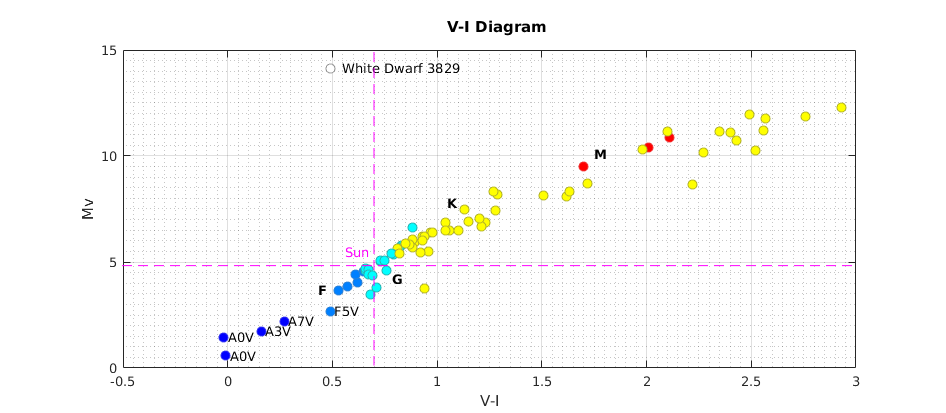
\includegraphics[width=15cm]{Figures/VIdiagram.png}
		\end{center}
		\caption{\footnotesize{En el siguiente diagrama se ha representado la relaci\'{o} entre la magnitud absoluta de cada estrella y su color V-I. Ambas cantidades est\'{a}n representadas en magnitudes.}}
		\label{VIdiag}
		\end{figure}

\hspace*{12pt} Como se puede observar en la Figura \ref{VIdiag} los resultados son muy similares a los obtenidos para el diagrama HR de la Figura \ref{HRdiag} excepto porque las diferencias entre la magnitud de las bandas V e I es mucho mayor (En magnitudes) que la diferencia entre las bandas B y V. Esto es debido a la forma de cuerpo negro que tiene la emisi\'{o}n estelar, en la cual una vez pasado el pico de emisi\'{o}n, situado cerca del V generalizando mucho, la curva del cuerpo negro cae de manera m\'{a}s abrupta que lo que sub\'{i}a antes del pico.

	\subsection{Diagrama Color - Color}
\hspace*{12pt} Los resultados obtenidos para el diagrama Color-Color son los que siguen (Ver Figura \ref{CCdiag}).

	\begin{figure}[!htbp]
		\centering
		\begin{center}
			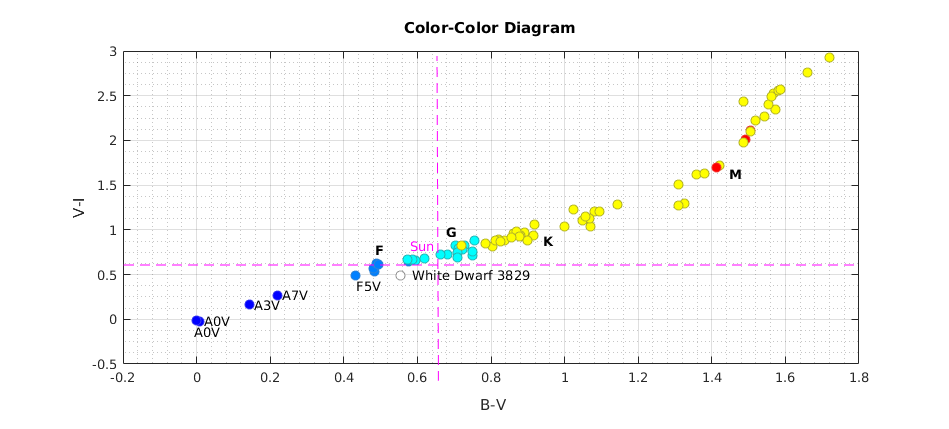
\includegraphics[width=15cm]{Figures/CC.png}
		\end{center}
		\caption{\footnotesize{En el siguiente diagrama se ha representado la relaci\'{o} entre el color B-V y el color V-I. Ambas cantidades est\'{a}n representadas en magnitudes.}}
		\label{CCdiag}
		\end{figure}
\hspace*{12pt} Como se puede observar en la Figura \ref{CCdiag} las estrellas se ordenan de forma creciente seg\'{u}n su orden espectral. Lo primero que conviene destacar es c\'{o}mo, efectivamente, las estrellas de tipo A0V se sit\'{u}an en el 0 de color para ambas bandas. Suponiendo estas estrellas como las m\'{a}s calientes, del diagrama se puede extraer informaci\'{o}n sobre  c\'{o}mo var\'{i}a la posici\'{o}n del pico de emisi\'{o}n con la temperatura de la estrella si esta es asemejable a un cuerpo negro. Seg\'{u}n el pico est\'{e} m\'{a}s azulado m\'{a}s caliente ser\'{a} la estrella. Esto queda reflejado en el color debido al cambio en la curva de emisi\'{o}n de la estrella.
\section{Estrellas fuera de la secuencia principal. Puntos destacables}
Las estrellas que, dentro del diagrama HR de la Figura \ref{HRdiag}, se salen (seg\'{u}n un criterio fundamentado pero en definitiva, subjetivo) de la secuancia principal y, por lo tanto, vamos a analizar por separado son las se\~{n}aladas en la Figura \ref{HRNum}.
	\begin{figure}[!htbp]
	\title{\textbf{Selecci\'{o}n de estrellas fuera de la secuencia principal} \vspace{3ex}}
		\centering
		\begin{center}
			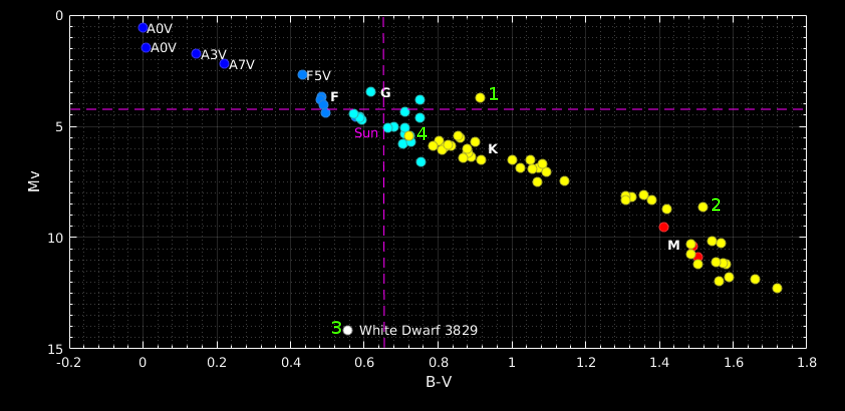
\includegraphics[trim={0 0.4cm 0 0},clip, width=15cm]{Figures/HRNumbers.png}
		\end{center}
		\caption{\footnotesize{Estrellas a analizar debido a su posici\'{o}n destacada en el diagrama}}
		\label{HRNum}
		\end{figure}
		
		\floatsetup[figure]{capposition=beside,capbesideposition={right,center}}
		
		
		\subsection{HIP 17378: Rana o del Eri.}
		\begin{figure}[H]
			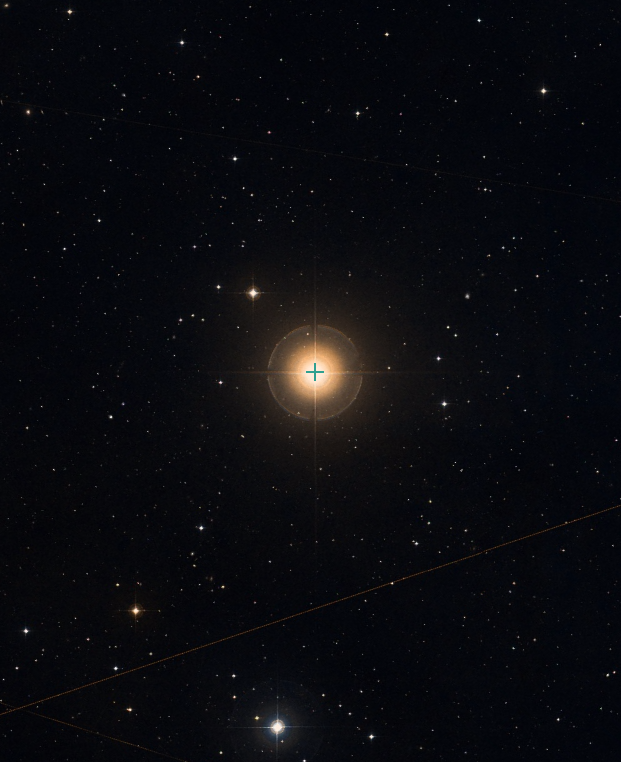
\includegraphics[trim={0 6cm 0 6cm},clip,width=6cm]{Figures/HIP17378.png}
			
			\caption{N\'{u}mero \textbf{1} en la Figura \ref{HRNum}. Su nombre gen\'{e}rico es Rana seg\'{u}n Antonin Becvar (1964) "Atlas of the Heavens - II: Catalogue 1950.0" o del Eri. Su posici\'{o}n en el diagrama HR se puede explicar mirando a su espectro de emisi\'{o}n el cual se asocia con una estrella de tipo IV, lo cual implica que est\'{a} comenzando su viaje por la rama de las gigantes.}
		\end{figure}
		
		
		\subsection{HIP 73182: Sistema Gliese 570, Gliese 570 A.}
				\begin{figure}[H]
			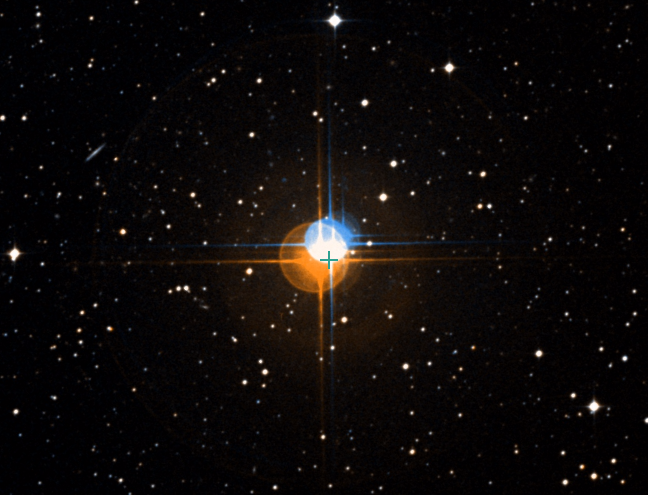
\includegraphics[width=6cm]{Figures/HIP73182.png}
			
			\caption{N\'{u}mero \textbf{2} en la Figura \ref{HRNum}. Este sistema se le conoce con el nombre gen\'{e}rico de Gliese 570. Se trata de un sistema cuaternario formado por un cuerpo central carcaterizado como enana naranja y dos estrellas,enanas rojas, que forman un sistema binario orbitando alrededor de la primera. Todo este sistema orbita a su vez alrededor de una estrella tipo K conocida como Gliese 570 A.}
		\end{figure}
		Debido a que la luminosidad que nos llega est\'{a} formada principalmente por las transiciones de la estrella tipo K el tipo espectral del sistema es el de Gliese 570 A. Sin embargo, se detecta una luminosidad mayor debido a que esta es la suma de las luminosidades de los objetos del sistema. Esto explica su posici\'{o}n en el diagrama HR por encima de las estrellas de tipo K solitarias.
		
		\subsection{HIP 3829: Wolf 28, La Enana Blanca.}
						\begin{figure}[H]
			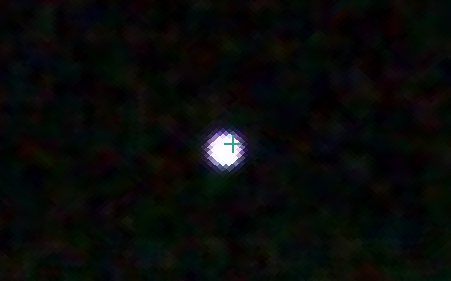
\includegraphics[width=6cm]{Figures/HIP3829.png}
			
			\caption{N\'{u}mero \textbf{3} en la Figura \ref{HRNum}. Esta estrella destaca en su posici\'{o}n en el diagrama HR debido a que es la \'{u}nica enana blanca en la vecindad solar, pero dentro del conjunto de las enanas coincide con la carcater\'{i}stica general de tener una luminosidad muy pequeña para la temperatura que tiene debido a su peque\~{n}o tama\~{n}o.}
		\end{figure}

		\subsection{HIP 72659: Ksi Boo.}
								\begin{figure}[H]
			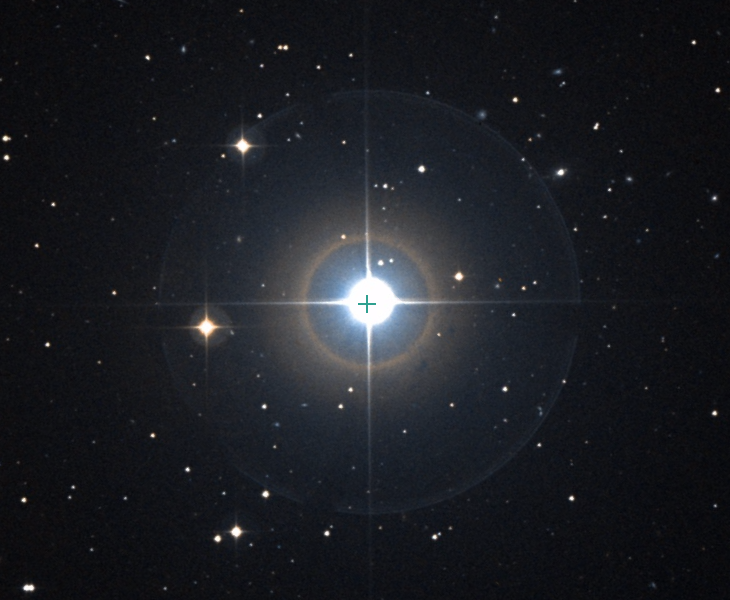
\includegraphics[trim={0 2cm 0 2cm},clip,width=6cm]{Figures/HIP72659.png}
			
			\caption{N\'{u}mero \textbf{4} en la Figura \ref{HRNum}. Este sistema se trata de un sistema binario de dos estrellas, una de tipo G y otra de tipo K. Aunque su color en el diagrama HR deber\'{i}a haber sido el de una estrella tipo G hemos querido destacarla para comentar m\'{a}s adelante su peculiaridad de estrella binaria.}
		\end{figure}

		



%\bibliographystyle{plain}
%\bibliography{bibliography.bib}

\end{document}
